\subsection{Question 1}

\begin{figure}[H]
  \centering
  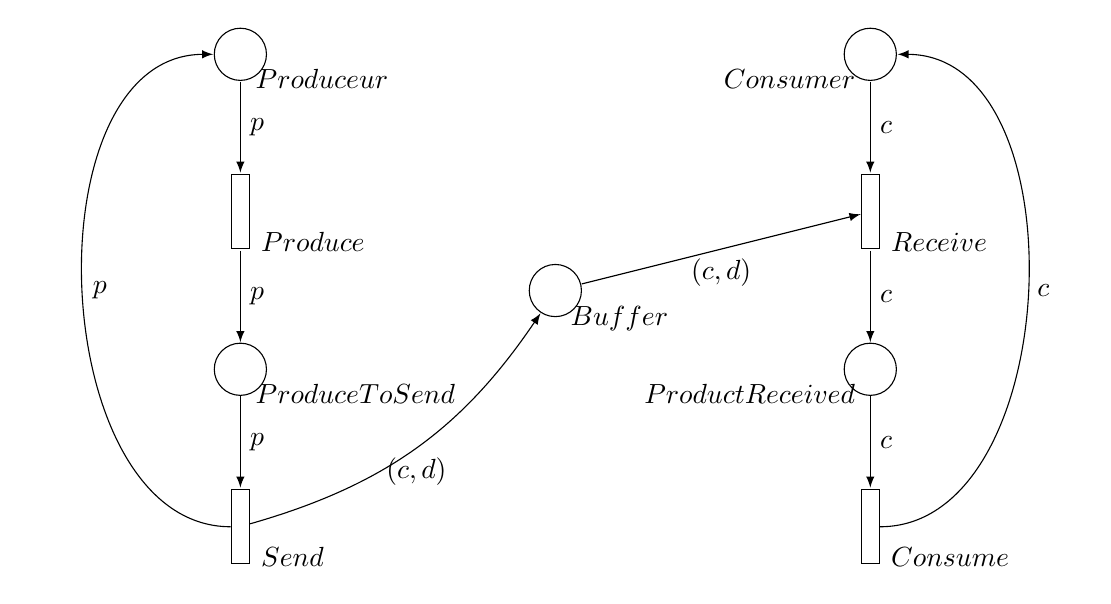
\begin{tikzpicture}

  	% Liste des places
    \draw (-4,3) node[below right = 2pt] {$Produceur$};
    \node[draw,circle,scale=2] (P) at (-4, 3) {};
    \draw (4,3) node[below left = 2pt] {$Consumer$};
    \node[draw,circle,scale=2] (C) at (4, 3) {};
    \draw (-4,-1) node[below right = 2pt] {$ProduceToSend$};
    \node[draw,circle,scale=2] (PtS) at (-4,-1) {};
    \draw (4,-1) node[below left = 2pt] {$ProductReceived$};
    \node[draw,circle,scale=2] (PR) at (4, -1) {}; %%
    \draw (0,0) node[below right = 2pt] {$Buffer$};
    \node[draw,circle,scale=2] (B) at (0, 0) {}; %%


     % Liste des transitions
    \draw (-4,1) node[below right = 4pt] {$Produce$};
    \node[draw,rectangle,yscale=4] (TP) at (-4, 1) {};
    \draw (-4,-3) node[below right = 4pt] {$Send$};
    \node[draw,rectangle,yscale=4] (TS) at (-4, -3) {};
    \draw (4,1) node[below right= 4pt] {$Receive$};
    \node[draw,rectangle,yscale=4] (TR) at (4, 1) {};
    \draw (4,-3) node[below right = 4pt] {$Consume$};
    \node[draw,rectangle,yscale=4] (TC) at (4, -3) {};

     % Liste des arcs
    \draw[->,>=latex] (P) -- (TP)node[midway, right]{$p$};
    \draw[->,>=latex] (TP) -- (PtS)node[midway, right]{$p$};
    \draw[->,>=latex] (PtS) -- (TS)node[midway, right]{$p$};
    \draw[->,>=latex] (TS) to[bend right = 20] node[midway, below]{$(c,d)$} (B);
    \draw[->,>=latex] (B) -- (TR)node[midway, below]{$(c,d)$};
    \draw[->,>=latex] (TS) to [out=180,in=180] node[midway, right]{$p$}(P);
    \draw[->,>=latex] (C) -- (TR)node[midway, right]{$c$};
    \draw[->,>=latex] (TR) -- (PR)node[midway, right]{$c$};
    \draw[->,>=latex] (PR) -- (TC)node[midway, right]{$c$};
    \draw[->,>=latex] (TC) to [out=0,in=0] node[midway, right]{$c$}(C);

    \end{tikzpicture}
  \caption{Réseau de petri coloré associé au protocole de production} \label{fig:M5}
\end{figure}

Lorsqu'un producteur crée un produit, un jeton avec une valeur $p$ est consommé en $Producer$ par $Produce$ et un jeton avec la même valeur est produit en $ProduceToSend$.
À ce moment là, la transition $Send$ consomme ce jeton de valeur $p$ en $ProduceToSend$ et va en produire 2, un dans $Producer$, avec la même valeur $p$,qui signifie que le producteur est à nouveau disponible, et un, en $Buffer$ avec un valeur double $(c,d)$ où $d$ correspond à la ``référence'' du produit et $c$ à son destinataire.
Ainsi, lorsque la transition $Receive$ sera sensibilisée, elle va associer le valeur $c$ du jeton $CONS$ consommé en $Consumer$ à la valeur $c$ contenu dans la paire du jeton $DATA$ consommé en $Buffer$.
Par conséquent, le reseau verifie que qu'un client consomme bien le produit qui lui est destiné.

\subsection{Question 2}

\begin{figure}[H]
  \centering
  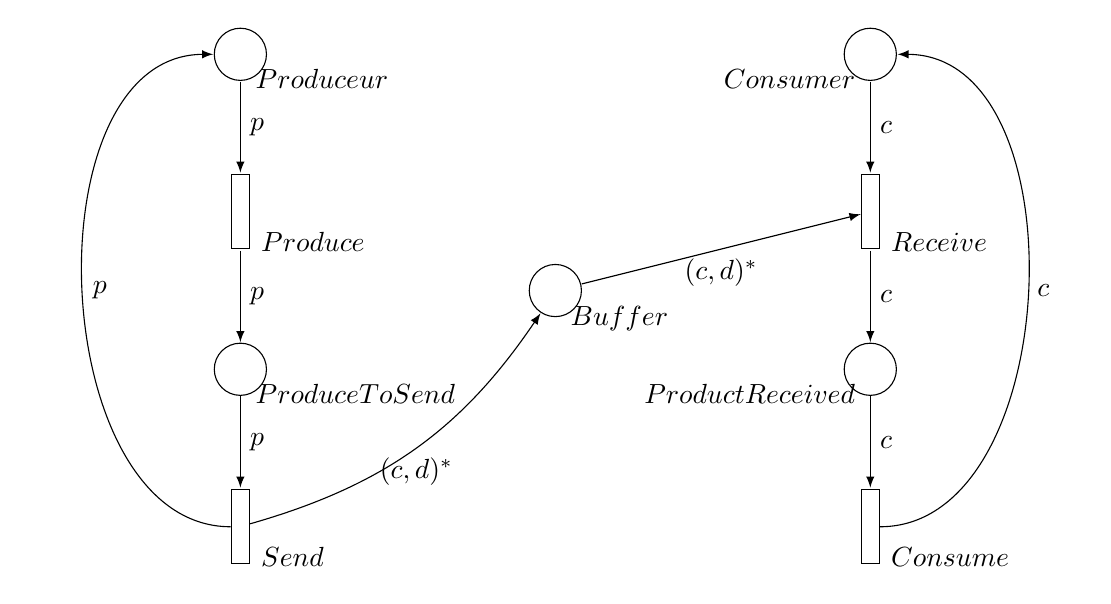
\begin{tikzpicture}

  	% Liste des places
    \draw (-4,3) node[below right = 2pt] {$Produceur$};
    \node[draw,circle,scale=2] (P) at (-4, 3) {};
    \draw (4,3) node[below left = 2pt] {$Consumer$};
    \node[draw,circle,scale=2] (C) at (4, 3) {};
    \draw (-4,-1) node[below right = 2pt] {$ProduceToSend$};
    \node[draw,circle,scale=2] (PtS) at (-4,-1) {};
    \draw (4,-1) node[below left = 2pt] {$ProductReceived$};
    \node[draw,circle,scale=2] (PR) at (4, -1) {}; %%
    \draw (0,0) node[below right = 2pt] {$Buffer$};
    \node[draw,circle,scale=2] (B) at (0, 0) {}; %%


     % Liste des transitions
    \draw (-4,1) node[below right = 4pt] {$Produce$};
    \node[draw,rectangle,yscale=4] (TP) at (-4, 1) {};
    \draw (-4,-3) node[below right = 4pt] {$Send$};
    \node[draw,rectangle,yscale=4] (TS) at (-4, -3) {};
    \draw (4,1) node[below right= 4pt] {$Receive$};
    \node[draw,rectangle,yscale=4] (TR) at (4, 1) {};
    \draw (4,-3) node[below right = 4pt] {$Consume$};
    \node[draw,rectangle,yscale=4] (TC) at (4, -3) {};

     % Liste des arcs
    \draw[->,>=latex] (P) -- (TP)node[midway, right]{$p$};
    \draw[->,>=latex] (TP) -- (PtS)node[midway, right]{$p$};
    \draw[->,>=latex] (PtS) -- (TS)node[midway, right]{$p$};
    \draw[->,>=latex] (TS) to[bend right = 20] node[midway, below]{$(c,d)^*$} (B);
    \draw[->,>=latex] (B) -- (TR)node[midway, below]{$(c,d)^*$};
    \draw[->,>=latex] (TS) to [out=180,in=180] node[midway, right]{$p$}(P);
    \draw[->,>=latex] (C) -- (TR)node[midway, right]{$c$};
    \draw[->,>=latex] (TR) -- (PR)node[midway, right]{$c$};
    \draw[->,>=latex] (PR) -- (TC)node[midway, right]{$c$};
    \draw[->,>=latex] (TC) to [out=0,in=0] node[midway, right]{$c$}(C);

    \end{tikzpicture}
  \caption{Réseau de petri coloré associé au protocole de production} \label{fig:M5}
\end{figure}

Dans ce cas, la production de produits n'est pas modifiée, seul l'envoie change.
Lors de l'envoie des produits,il vont être rassembler dans un liste finie (type FIFO). Cette liste est alors envoyée et reçu sans modification.
Ainsi le premier élément qui devait être envoyé sera le premier à être mis dans la liste avant son envoie et également le premier à être pris dans la listeaprès sa réception.
Donc, grace à ce système, l'ordre d'envoie et de reception sont identique.
